\documentclass[a4paper]{article}
\usepackage[applemac]{inputenc}
\usepackage{xcolor}
\usepackage{graphicx}
\usepackage{amssymb}
\usepackage{a4wide}
\usepackage{stringstrings}
\usepackage{titling}
\usepackage[pdftex,colorlinks=true,pdfstartview=FitV,linkcolor=black,citecolor= black,urlcolor= black]{hyperref}
\usepackage{ifthen}
\usepackage{fancyhdr}

%%%%%%%%%%%%%%%%%%%%%%%%%%%%%%%%%%%%%%%%%%%%%%%%%%%%%%%%%%%%
\pdfinfo{
  /Title(Curriculum Vitae)
  /Author(Mircea F. Lungu)
  /Subject()
  /Keywords($Id$)
}
%%%%%%%%%%%%%%%%%%%%%%%%%%%%%%%%%%%%%%%%%%%%%%%%%%%%%%%%%%%%
\begin{document}
\title{\textsf{Mircea F. Lungu, PhD \\Curriculum Vit\ae}}
\author{}

\pagestyle{myheadings}
\pagestyle{fancy}

\thispagestyle{plain}

\renewcommand{\headrulewidth}{0.0pt}
\renewcommand{\footrulewidth}{0.0pt}

\lfoot{M.F. Lungu, CV}

\posttitle{\par\end{center}\vspace{-1.0cm}}
\date{\today\\\small http://mir.lu/cv}
\maketitle

\thispagestyle{empty}


%%%%%%%%%%%%%%%%%%%%%%%%%%%%%%%%%%%%%%%%%%%%%%%%%%%%%%%%%%%%

% \vspace{-4cm}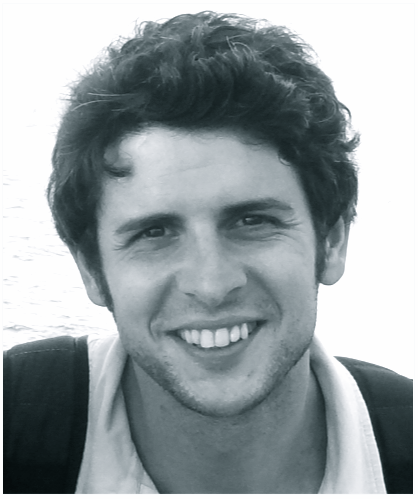
\includegraphics[width=3cm]{ml-bw.png}
% \vspace{0.5cm}


\newcommand{\cvsection}[1]{\section*{\capitalizetitle{#1}}\vspace{-0.75em}\hrule\vspace{1em}}


% Empirical Software Engineering, 
% Software evolution,
% Reverse and re-engineering,
% Programming Languages,
% Triathlon, Music, Theatre.

\newcommand{\job}[4]{#1 & {\bf #3}\\ & #2\\  &{\small \em#4} \vspace{0.5em} \\}
%%%%%%%%%%%%%%%%%%%%%%%%%%%%%%%%%%%%%%%%%%%%%%%%%%%%%%%%%%%%
\cvsection{Experience}

\begin{tabular}{r p{8cm}}

	\job
	{2015 -- present}
	{Johann Bernoulli Institute for Mathematics and Computer Science at the University of Groningen}
	{Assistant Professor}
	{Teaching and Conducting research in software evolution}

	\job
	{2010 -- 2015}
	{Computer Science Institute, University of Bern}
	{Researcher \& Lecturer}
	{
	%Assisting Oscar Nierstrasz in managing the SCG. 
	Conducting research in SE and programming languages. Mentoring graduate students. Teaching.}

	\job
	{2012}
	{Department of Informatics, UC Irvine}
	{Visiting Researcher}
	{Collaborative research in software evolution. 
	% Integrating Softwarenaut and Sourcerer
	}


	\job
	{2009 -- 2010}
	{Faculty of Informatics, University of Lugano}
	{Postdoctoral Researcher}
	{Conducting research in software evolution. }

	\job 
	{Jul -- Dec, 2007}
	{IBM TJ Watson Research Center, NY}
	{Visiting Researcher}
	{Visualizing distributed systems with Wim De Pauw}


	\job 
	{2004 -- 2009}
	{Faculty of Informatics, University of Lugano}
	{PhD Student}
	{Conducting research in software evolution, visualization, and large scale software analysis}


	\job
	{2001 -- 2003}
	{Computervoice Systems, Timisoara, RO}
	{Software Engineer}
	{Writing customer management software for several telecommunication companies from the US}

	% \job
	% {1999 -- 2001}
	% {Logos Professional Highschool, Timisoara, RO}
	% {Instructor}
	% {Teaching Introduction to Programming with Pascal}

\end{tabular}




\newcommand{\degree}[5]{ \hspace{1.6cm}#2 & {\bf #1}\\ & #3\\ &#4\\ &#5\\ \\}
%%%%%%%%%%%%%%%%%%%%%%%%%%%%%%%%%%%%%%%%%%%%%%%%%%%%%%%%%%%%
\cvsection{Education}

\begin{tabular}{ r p{11cm}}

\degree
	{PhD}
	{2009}
	{Faculty of Informatics, University of Lugano}
	{Dissertation: {\em Reverse Engineering Software Ecosystems}}
	{Advisor: Prof. Dr. Michele Lanza}

\degree
	{Dipl. -Ing.}
	{2004}
	{Computer Science Department, Polytechnic University of Timisoara}
	{Thesis: \emph{Conformity Strategies - Measures of Software Design Rules}}
	{Supervisors: Prof. Dr. Radu Marinescu, Dr. Tudor G\^irba}

\end{tabular}


\newpage
%!TEX root = resume-long.tex

\cvsection{Honours and Awards (Selected)}
\newcommand {\award}[3]{\makebox[3.5cm][r]{\small #3} & {\bf #1} \\ & #2 \vspace{0.7em}\\}

\begin{tabular}{rp{10.5cm}}

	\award
		{OOPSLA Best Reviewer Award}
		{The ACM SIGPLAN Conference on Systems, Programming, Languages and Applications}
		{2013}

	\award 
		{Vice-President of CHOOSE}
		{The Swiss Group for Object Oriented Systems and Environments}
		{}

	\award
		{Best Paper Award}
		{With Lile Hattori at IWPSE-EVOL 2010 for {\em Replaying Past Changes in Multi-Developer Projects}}
		{2010}

	\award
		{1st Place}
		{ESUG Innovation Awards for the {\em Small Project Observatory} a platform for the visualization, monitoring, and analysis of software ecosystems}
		{2007}

	% \award
	% 	{Best Poster Award}
	% 	{The 3rd International ACM Symposium on Software Visualization, Brighton 2006, for the poster {\em Cutting Edge Software Visualization}}
	% 	{2006}

	\award
		{Best Software Engineer Award}
		{The Software Engineering Project at the Polytechnic University of Timisoara, RO}
		{2003}

	\award
		{2nd Place}
		{With {\em UPT} for building an image processing-based security system in 48 hours International {\em Hard \& Soft} Competition, Suceava, RO}
		{2002}

	% \award
	% 	{3rd Place}
	% 	{The National Student Software Development Contest, Focsani, RO}
	% 	{1999}

\end{tabular}




%


%!TEX root = CV_Publist_MirceaLungu.tex

\cvsection{Invited Talks}
Conference presentations are not included.
\vspace{1em}

\newcommand {\talk}[4]{\makebox[3cm][r]{\small #4} & {\bf #1} \\ & #3 (#2) \vspace{0.75em} \\}

\begin{tabular}{rp{10.5cm}}
	
	\talk 
		{Program Comprehension Across Levels of Abstraction}
		{Invited Talk}
		{University of California, Irvine}
		{May, 2013}

	\talk
		{Software is Data Too}
		{Keynote}
		{Smalltalks 2012, Argentina}
		{Nov, 2012}

	\talk
		{What do I talk about when I talk about Software Ecosystems}
		{Invited Talk}
		{University of Buenos Aires}
		{}	

	\talk 
		{Reverse Engineering Software Ecosystems}
		{Invited Talk}
		{University of California, Irvine}
		{Jul, 2011}

	\talk
		{Ecosystem Analysis}
		{Invited Talk}
		{PL'10: The 3$^{rd}$ Summer School on Programming Languages}
		{Nov, 2010}

	\talk
		{Architecture Recovery}
		{Guest Lecture}
		{University of Lugano}
		{Sep, 2010}

	\talk
		{Web-based visualization tools for reverse engineering}
		{Invited Talk}
		{2nd International Workshop on Advanced Software Development Tools and Techniques, Beijing}
		{Oct 2008}

	\talk 
		{The Small Project Observatory}
		{Invited Talk}
		{IBM TJ Watson Research Center}
		{Nov, 2007}
\end{tabular}




%!TEX root = resume-long.tex
\newcommand {\conf}[3]{ $^{ #2}$ #1  & #3  \\}
\newcommand {\activity}[4]{$^{ #2}$ #1  & #3 \\ & {\em \small #4} \vspace {0.5em}\\}
\newcommand {\event}[4]{\activity{#1}{#2}{#3}{#4}}


\newcommand {\track}[1]{ \emph{(#1)}}
\newcommand {\tdtrack}{\track{TD} }
\newcommand {\eratrack}{\track{ERA} }
\newcommand {\tderatrack}{\track{TD,ERA} }
\newcommand {\tablesection}[1]{\\ \\ & \multicolumn{1}{l}{\bf  #1} \vspace{0.5em}\\}
\newcommand {\contrib}[1]{\hspace{1em} #1\\}


\cvsection{Professional Activities (Selected)}
% Corresponding years are superscripted where available.

\begin{tabular}{rp{10.4cm}}


\tablesection{Project Writer}

	\conf{ASA}{`13}{\href{http://p3.snf.ch/Project-144126}{Agile Software Assessment} -- project co-written with Oscar Nierstrasz funded by the Swiss NSF (project \# 200020-144126/1)}


\tablesection{External Expert}

	\conf{NWO}{}{Netherlands Organization for Scientific Research}
	\conf{EU}{}{European Commission's FP7 Programme}


\tablesection{Program Chair}

	\conf{VISSOFT}{`14}
	{IEEE Working Conference on Software Visualization \eratrack}

	\conf{CSMR}{`12}
	{European Conference on Maintenance \& Reengineering \tdtrack}

	\conf{WCRE}{`11}
	{International Conference on Reverse Engineering \tdtrack}

\tablesection{Co-Organizer}
 
	\event
		{CHOOSE Forum}
		{`12, `13, `14}
		{Yearly event that brings together the SE Industry and Research}
		{with Tudor Girba and Michele Lanza (University of Lugano)}

	\event
		{WEA}{`13, `14} 
		{International Workshop on Software Ecosystem Architectures}
		{with Jens Knodel (Fraunhofer Institute)}

	\event
		{SATTOSE}{`13} 
		{Seminar on Advanced Techniques in Software Engineering}
		{with Oscar Nierstrasz (University of Bern)}

	\event
		{USI PhD Talks}{`06 - `09}
		{Weekly interdisciplinary research presentations}
		{with Cyrus Hall}


\tablesection{Journal Reviewer}

	\conf{TSE}{}{IEEE Transactions on Software Engineering} % 2014

	\conf{JSME}{}{Software Maintenance and Evolution} % 2012 

	\conf{EMSE}{}{Empirical Software Engineering}

	\conf{JSS,SCP}{}{Elsevier: Systems and Software, Science of Computer Programming}

	% \conf{SCP}{}{Elsevier }

	% \conf{FTHCI}{}{Foundations and Trends in Human Computer Interaction}

	\conf{IEEE Software}{}{The IEEE Software Magazine}
 



\tablesection{Conference PC Member}

	\conf{SANER}{`15}{22nd Int. Conf. on Software Analysis, Evolution and Reengineering}

	\conf{OOPSLA}{`13}{Conference on Systems, Programming, Languages and Applications}

	\conf{ICSE}{`12, `14}{Int. Conf.  on Software Engineering \tdtrack}

	\conf {ICPC}{`14}{Int. Conf.  on Program Comprehension}

	\conf{WCRE}{`12, `13, `14}{Int. Conf.  on Reverse Engineering}

	\conf{ICSME}{`11, `12, `14}{Int. Conf. on Software Maintenance \& Evolution\tderatrack}


	\conf{MSR}{`14, 15}{Int. Conf. om Mining Software Repositories}
	% \conf{WASDeTT}{`11, `13}{Workshop on Advanced Software Development Tools and Techniques}

	\conf{ESEC/FSE}{`11}{European Software Engineering/ACM SIGSOFT Symposium on the Foundations of Software \tdtrack}


% \end{tabular}
% 2014 & WCRE + CSMR, ICSE (TD Track)\\
% 2013 & OOPSLA, WCRE, WASDeTT, CSMR, ICSM (TD Track) \\
% 2012 & ICSE (Posters \& TD Track), WCRE, ICSM (TD Track), CSMR \\
% 2011 & ICSM (TD Track), WASDeTT, ESEC/FSE 2011 (TD Track), CSMR, IWPSE/EVOL\\
% 2010 & IWSECO, WSE\\





\end{tabular}






% \subsubsection*{Member Of Professional Organizations}
% CHOOSE - Swiss Group for Object Oriented Systems and Environments \footnote{\url{http://choose.s-i.ch}} 2011 - present.




% \newcommand {\lecture}[3]{{\small #3} & {\bf #1} \\ & #2 \vspace{0.7em}\\ }
\newcommand {\lecture}[3]{\item {\bf #1}\\#2, #3 }
\newcommand {\ub}{University of Bern}
\newcommand {\ul}{University of Lugano}
\newcommand {\msc}{MSc, }
\newcommand {\bsc}{BSc, }

\cvsection{Undergraduate and Graduate Lectures}
\begin{enumerate}
	\lecture{Software Engineering}{\bsc \ub}{Fall 2013, Fall 2014}
	\lecture {Compiler Construction}{\msc \ub}{Spring 2013}
	\lecture {Concurrency: State Models and Design Patterns}{\msc \ub}{Fall 2012}
	\lecture {Software Design and Evolution}{\msc \ub}{Spring 2012, Fall 2014}
	\lecture {Principles of GUI Design}{\bsc \ul}{\bsc Spring 2011}
	\lecture {Human Computer Interaction}{\bsc \ul}{2008}
	\lecture {Programming Fundamentals (I+II)}{\bsc \ul}{2005 -- 2007, (Teaching Assistant)}

\end{enumerate}


%!TEX root = resume-long.tex
\cvsection{Supervised Theses (Selected)}

\newcommand{\super}[5]{\item {\bf #2}\\ #1. #3, #4 #5}
\newcommand{\inprogr}{{\footnotesize(in progress)}}
\newcommand{\inprogrcosup}{{\footnotesize(in progress, co-supervised with O. Nierstrasz)}}

\newcommand{\yr}[1]{(#1)}

These are several of the theses (BSc, MSc, PhD) that I supervised or co-supervised over the years:

\begin{enumerate}

% \super 
% 	{G. Digkas}
% 	{Technical Debt }
% 	{PhD}
% 	{Groningen}
% 	{\inprogrcosup}

\super 
	{A. Caracciolo}
	{Agile Specification of Architectural Constraints}
	{PhD}
	{Bern}
	{2016}

\super 
	{J. Kurs}
	{Agile Parsing}
	{PhD}
	{Bern}
	{\inprogrcosup}	

\super 
	{B. Spasojevi\'{c}}
	{Mining the Ecosystem to Improve Developer Tools}
	{PhD}
	{Bern}
	{\inprogrcosup}

\super 
	{H. Osman}
	{Fine Grained Bug Pattern Detection and Prediction}
	{PhD}
	{Bern}
	{\inprogrcosup}	



\super 
	{D. Rahm}
	{Hikomsys: Gamifying Software Analysis}
	{BSc}
	{Bern}
	{2015}

% \super 
% 	{B. Aga}
% 	{Automatically Breaking Dependency Cycles}
% 	{MSc}
% 	{Bern}
% 	{\inprogr}

\super 
	{D. Schenk}
	{Quicksilver: A Framework for Hierarchical Data Analysis}
	{MSc}
	{Bern}
	{\yr{2014}}

\super 
	{N. Haenni}
	{Developer Information Needs in Software Ecosystems}
	{MSc}
	{Bern}
	{\yr{2014}}

\super 
	{S. Marti}
	{Second Language Acquisition Through Free Reading and Repetition}
	{BSc}
	{Bern}
	{\yr{2013}}

\super 
	{E. Aeschlimann}
	{St1-PL/1
Extracting quality information from PL/1 legacy ecosystems}
	{MSc}
	{Bern}
	{\yr{2013}}


% \super 
% 	{A. Bockmann}
% 	{Modular Architecture Recommendation System}
% 	{MSc}
% 	{Lugano}
% 	{\yr{2010}}

\super 
	{J. Malnati}
	{Developer-Centric Analysis of SVN Ecosystems}
	{MSc}
	{Lugano}
	{\yr{2009}}


% \item Jacopo Malnati. \emph{X-Ray - An Eclipse Plug-in for Software Visualization}. Bachelor Thesis, University of Lugano, 2007.

\end{enumerate}

%%%%%%%%%%%%%%%%%%%%%%%%%%%%%%%%%%%%%%%%%%%%%%%%%%%%%%%%%%%%
\newpage
\newcommand{\paper}[3]{\item \emph{\bf #1}\\#2\\In #3}

\newcommand{\densepaper}[3]{\item \emph{\bf #1. }#2. In #3}

\newcommand{\densepap}[6]{\item \emph{\bf #1}\\#2\\ In #3, p. #4. #6}

\newcommand{\ieee}{IEEE Computer Society}
\newcommand{\IEEE}{\ieee}


\cvsection{Peer-Reviewed Publications (Selected)}

\emph{H-index:} 15.
These and further publications are available online at \url{http://scg.unibe.ch/staff/mircea/pubs} or on \href{http://scholar.google.ch/citations?user=7zx6Cg0AAAAJ}{the Google Scholar website.}

\subsubsection*{Journal Articles}
	%!TEX root=CV_Publist_MirceaLungu.tex
%%%%%%%%%%%%%%%%%%%%%%%%%%%%%%%%%%%%%%%%%%%%%%%%%%%%%%%%%%%%

% ==========================================================
\begin{enumerate}

\paper
	{Predicting dependences using domain-based coupling}
	{Amir Aryani, Fabrizio Perin, Mircea Lungu, Abdun Naser Mahmood, and Oscar Nierstrasz}
	{Journal of Software: Evolution and Process 26(1), p. 50-76, 2014}

\paper 
	{Evolutionary and Collaborative Architecture Recovery with Softwarenaut}
	{Mircea Lungu, Michele Lanza, and Oscar Nierstrasz.}
	{Science of Computer Programming 79(0) p. 204 - 223, 2014}

\paper 
	{Answering software evolution questions: An empirical evaluation}
	{Lile Hattori, Marco D'Ambros, Michele Lanza, and Mircea Lungu}
	{Information and Software Technology 55(4) p. 755 - 775, January 2013}

\paper 
	{Incremental Dynamic Updates with First-class Contexts}
	{Erwann Wernli, Mircea Lungu, and Oscar Nierstrasz}
	{Journal of Object Technology 12(3) p. 1:1-27, 2013}

\paper
	{Seuss: Decoupling  static method responsibilities for fine-grained configurability}
	{Niko Schwarz, Mircea Lungu, and Oscar Nierstrasz}
	{Journal of Object Technology 11(1), 2012}

\paper 
	{On Porting Software Visualization Tools to the Web}
	{Marco D'Ambros, Michele Lanza, Mircea Lungu, and Romain Robbes}
	{Journal on Software Tools for Technology Transfer 13 p. 181 -- 200, 2011}

\paper 
	{The Small Project Observatory: Visualizing Software Ecosystems}
	{Mircea Lungu, Michele Lanza, Tudor G\^irba, and Romain Robbes}
	{Science of Computer Programming, Elsevier 75(4) p. 264-275, 2010}

\paper 
	{Visualizing Co-Change Information with the Evolution Radar}
	{Marco D'Ambros, Michele Lanza, and Mircea Lungu}
	{Transactions on Software Engineering (TSE) 35(5) p. 720 - 735, 2009}

\end{enumerate}






\subsubsection*{Refereed Papers in International Conferences}
	%!TEX root = resume-long.tex
\begin{enumerate}


\densepap
	{Mining frequent bug-fix code changes}
	{Haidar Osman, Mircea Lungu, and Oscar Nierstrasz}
	{(CSMR-WCRE'14) Proceedings of the IEEE Conference on Software Maintenance, Reengineering and Reverse Engineering }
	{343--347}
	{2014}
	{\IEEE}

\densepap 
	{On how often code is cloned across repositories}
	{Niko Schwarz, Mircea Lungu, and Romain Robbes}
	{(ICSE'12) Proceedings of the 34th International Conference on Software Engineering }
	{1289--1292}
	{2012}
	{\IEEE}

\densepap
	{How Do Software Architects Specify and Validate Quality Requirements?}
	{Andrea Caracciolo, Mircea Lungu, Oscar Nierstrasz}
	{(ECSA'14) Proceedings of the 8th European Conference on Software Architecture }
	{374 -- 389}
	{2014}
	{Springer LNCS Vol. 8627}

\densepap
	{Mining the Ecosystem to Improve Type Inference for Dynamic Languages}
	{Boris Spasojevic, Mircea Lungu, Oscar Nierstrasz}
	{(Onward! '14) Proceedings of the 2014 ACM International Symposium on New Ideas, New Paradigms, and Reflections on Programming \& Software }
	{133--142}
	{2014}
	{ACM}

\densepap
	{Bounded Seas -- Island Parsing Without Shipwrecks}
	{Jan Kurs, Mircea Lungu, Oscar Nierstrasz}
	{(SLE'14) Proceedings of the 7th International Conference on Software Language Engineering }
	{62--81}
	{2014}
	{LNCS Vol. 8706}

\densepap
	{Analyzing PL/1 legacy ecosystems: An experience report}
	{Erik Aeschlimann, Mircea Lungu, Oscar Nierstrasz, Carl F. Worms}
	{(WCRE'13) Proceedings of the 20th Working Conference on Reverse  Engineering }
	{441--448}
	{2013}
	{\IEEE}

\densepap
	{How Do Developers React to API Deprecation?}
	{Romain Robbes, Mircea Lungu, and David Roetlisberger}
	{(FSE'12) Proceedings of the 20th International Symposium on the Foundations of Software Engineering }
	{56:1 -- 56:11}
	{2012}
	{ACM}

\densepap
	{On How Often is Code Cloned Across Repositories}
	{Niko Schwarz, Mircea Lungu, and Romain Robbes}
	{(ICSE'12) Proceedings of the 34th International Conference on Software Engineering }
	{1289--1292}
	{2012}
	{\IEEE}

\densepap
	{Incremental Dynamic Updates with First-class Contexts}
	{Erwann Wernli, Mircea Lungu, and Oscar Nierstrasz}
	{(TOOLS'12) Proceedings of the 50th international conference on Objects, Components, Models and Patterns}
	{304--319}
	{2012}
	{LNCS Vol. 7304}


% \item Amir Aryani, Fabrizio Perin, Mircea Lungu, Abdun Naser Mahmood, and Oscar Nierstrasz. \emph{Can We Predict Dependencies Using Domain information?.} In Proceedings of the 18th Working Conference on Reverse Engineering (WCRE 2011), October 2011. 

% \densepap
% 	{Erase and rewind  --  Learning by replaying examples}
% 	{Lile Hattori and Alberto Bacchelli and Michele Lanza and Mircea Lungu}
% 	{Proceedings of the 24th Conference on Software Engineering Education and Training (CSEET)}
% 	{}
% 	{2011}
% 	{}


\densepap
	{Software Evolution Comprehension: Replay to the Rescue}
	{Lile Hattori, Marco D'Ambros, Michele Lanza, and Mircea Lungu}
	{(ICPC'11) Proceedings of the 19th International Conference on Program Comprehension }
	{161--170}
	{2011}
	{\IEEE}

% \densepap
% 	{A Study of Ripple Effects in Software Ecosystems}
% 	{Romain Robbes and Mircea Lungu}
% 	{Proceedings of the 33rd International Conference on Software Engineering (ICSE 2011)}
% 	{904--907}
% 	{May 2011}
% 	{}


\densepap
	{Flexible object layouts: language extensions by intercepting slot access}
	{Toon Verwaest, Camillo Bruni, Mircea Lungu, and Oscar Nierstrasz}
	{(OOPSLA '11) Proceedings of the 2011 ACM international conference on Object oriented programming systems languages and applications }
	{959--972}
	{2011}
	{ACM}

% \densepap
% 	{Recovering Inter-Project Dependencies in Software Ecosystems}
% 	{Mircea Lungu, Romain Robbes, and Michele Lanza}
% 	{Proceedings of the 25th IEEE/ACM International Conference on Automated Software Engineering (ASE'10)}
% 	{}
% 	{2010}
% 	{ACM Press}


% \item Marco D'Ambros, Mircea Lungu, Michele Lanza, and Romain Robbes. \emph{Promises and Perils of Porting Software Visualization Tools to the Web.} In Proceedings of WSE 2009 (11th IEEE International Symposium on Web Systems Evolution), p. 109-118, IEEE CS Press, 2009.

\densepap
	{Exploring Inter-Module Relationships in Evolving Software Systems}
	{Mircea Lungu and Michele Lanza}
	{(CSMR '07) Proceedings of the 11th European Conference on Software Maintenance and Reengineering }
	{91--100}
	{2007}
	{\IEEE}

\densepap
	{Reverse Engineering Super-Repositories}
	{Mircea Lungu, Michele Lanza, Tudor G\^irba, and Reinout Heeck}
	{(WCRE '07) Proceedings of th 14th Working Conference on Reverse Engineering}
	{120--129}
	{2007}
	{\IEEE}

\densepap
	{An Approach to Software Evolution Based on Semantic Change}
	{Romain Robbes, Michele Lanza, and Mircea Lungu}
	{(FASE '07) Proceedings of 10th International Conference on Fundamental Approaches to Software Engineering}
	{27--41}
	{2007}
	{Springer}


\densepap
	{Mondrian: An Agile Visualization Framework}
	{Michael Meyer, Tudor G\^irba, and Mircea Lungu}
	{(SoftVis '06) ACM Symposium on Software Visualization}
	{135--144}
	{2006}
	{ACM}

\end{enumerate}






\newpage
\newcommand{\reference}[4]{{\bf #1}\\#2\\#3 \\ \\}
\cvsection{References}
%%%%%%%%%%%%%%%%%%%%%%%%%%%%%%%%%%%%%%%%%%%%%%%%
\begin{tabular}{p{10cm}}

\reference
	{Prof. Dr. Cristina Videira Lopes}
	{School of Information and Computer Sciences\\University of California Irvine}
	{lopes@ics.uci.edu}

\reference
	{Prof. Dr. Mehdi Jazayeri}
	{Faculty of Informatics\\University of Lugano}
	{mehdi.jazayeri@usi.ch}

\reference
	{Prof. Dr. Harald Gall}
	{Software Architecture Lab\\University of Zurich}
	{gall@ifi.uzh.ch}

\reference
	{Prof. Dr. Oscar Nierstrasz}
	{Software Composition Group\\University of Bern}
	{oscar@iam.unibe.ch}

\reference
	{Prof. Dr. Michele Lanza}
	{Faculty of Informatics\\University of Lugano}
	{michele.lanza@usi.ch}



% \reference
% 	{Dr. Wim de Pauw}
% 	{Google Inc.\\Ex: IBM T.J. Watson Research Center}
% 	{Email: wim@us.ibm.ch}

% \reference
% 	{Prof. Dr. Radu Marinescu}
% 	{Faculty of Computer Science\\Polytechnic University of Timisoara}
% 	{Email: radum@cs.utt.ro}


% \reference
% 	{Dipl. Ing. Calin Sircuta}
% 	{\\Computervoice Systems, Romania. 
% \\Email: sircux@computervoice.ro\\}
	
\end{tabular}


\cvsection{Personal Information} % (fold)
\label{sec:further_relevant_information}

\begin{tabular}{p{3cm}l}
	Natural Languages		& Romanian, English, French, Italian, German \\
	Sports			& Triathlon, Tennis \\
	Volunteering	& Co-Founder of Lifelong Education Foundation
\end{tabular}



\cvsection{Contact}
\begin{tabular}{p{10cm}}

Institut f�r Informatik (IAM)\\Universit�t Bern \\
Neubr�ckstrasse 10, CH-3012\\ Bern, Switzerland \\ \\
+41 31 631 7637 (Office) \\
+41 31 631 3355 (Fax) \\
\href{mailto:lungu@iam.unibe.ch}{lungu@iam.unibe.ch} \\ \\
\end{tabular}

%Birthdate		& October 24, 1980 (Arad, Romania)\\
%Citizenship		& Romanian \\
%Name				& Mircea Filip Lungu \\
%Residence		& Z�hringerstrasse 78, Bern\\
%Mobile			& +41 78 904 3235\\




% \input{refs}
\end{document}
%%%%%%%%%%%%%%%%%%%%%%%%%%%%%%%%%%%%%%%%%%%%%%%%%%%%%%%%%%%%
